\section{Conclusion}

%1: answer RQs
The current body of knowledge is severely lacking in both academia and industry. We found only two papers \cite{Sanjay2011,Garcia2010} doing performance tests in academia and a larger number of outdated and biased industrial papers \cite{Perera07,Perera07R2,Perera07R3,mulesoft08}.
There is enough papers for us to at least get a foundation of testing to build upon which is what we do in our test framework. The framework consists of a series of scenarios aimed at testing the core functionality of any ESB and we have used Mule ESB as verification that the framework works as expected. 

%2:	our contribution
The largest conclusion done in this thesis is that the current body of knowledge seems to be severly lacking in both industry and academia. 
Most importantly the paper we have found \cite{Sanjay2011} lack a reproducibility which is, possibly, even more important than an unbiased test. 
We have also started a humble attempt at creating a testing framework that could serve as a foundation for future tests. 
Below is an analysis of some of the other tests performed byt others and how they compare to our results.


\newpage
%snacka om industrins grafer
\begin{figure}[H]
	\caption{Image taken from WSO2s test \cite{Perera07R3} showing their content based routing measurements.}
	\centerline{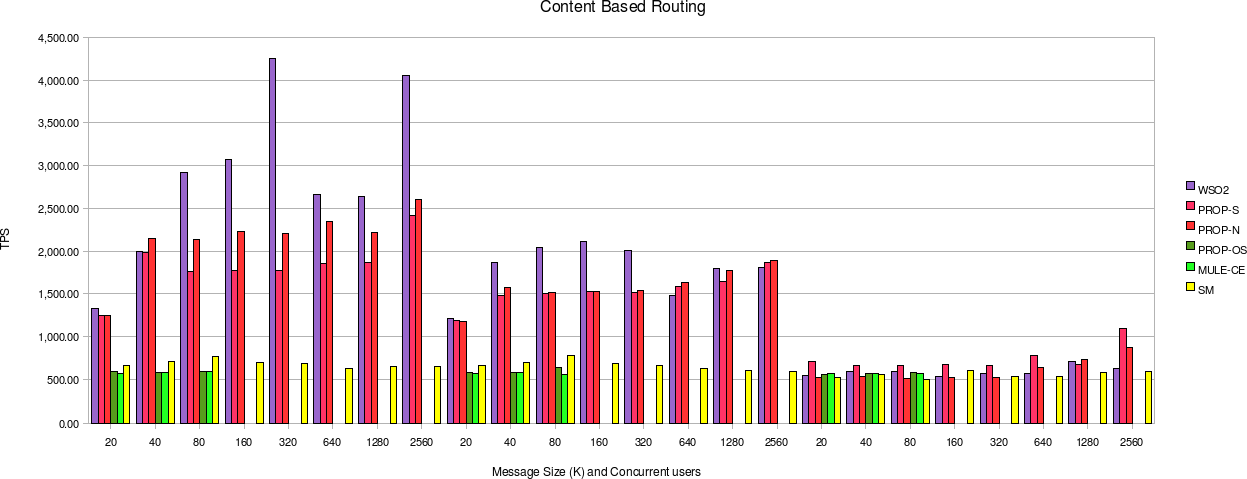
\includegraphics[scale=0.43]{img/WSO2_cbr_chart}}
	\label{fig:wso2_cbr}
	Payload is increasing (0.5KB, 1KB and 5KB) and the X-axis is numbers of clients sending data. 
	All values seem to be above 500TPS with some tests not being able to complete on all ESB solutions.

	\caption{Image taken from Mules test \cite{mulesoft08} showing their content based routing measurements.}
	\centerline{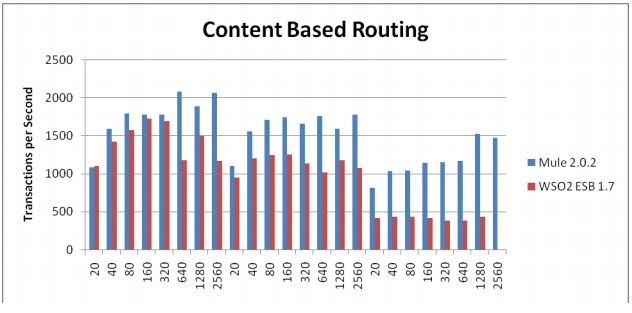
\includegraphics[scale=1]{img/MULE_cbr_chart}}
	\label{fig:mule_cbr}
	Payload is increasing (0.5KB, 1KB and 5KB) and the X-axis is numbers of clients sending data. 
\end{figure}
While looking at figure \ref{fig:wso2_cbr} we can clearly see that Mule has failed the majority of tests performed by WSO2 \cite{Perera07R3}. 
It is therefore not suprising that in the following figure from Mules test \cite{mulesoft08} shows WSO2 failing tests and performing far below Mule.

What is most suprising to us is that in these tests the TPS is above 500TPS and often above 1000TPS overall. 
If we look at the second "20" mark on the x-axis which is 1KB sent by 20 concurrent users both WSO2 and Mules tests show values between 500TPS and 1000TPS while in our own tests with an ESB didn't even break 10TPS.
Even without an ESB we could not achieve such high numbers which could mean that the configuration of grinder or the webservice needs to be finetuned.

\newpage
%snacka om sanjays grafer
\begin{figure}[H]
	\caption{Image taken from Sanjay \cite{Sanjay2011} showing their fixed payload content based routing measurements.}
	\centerline{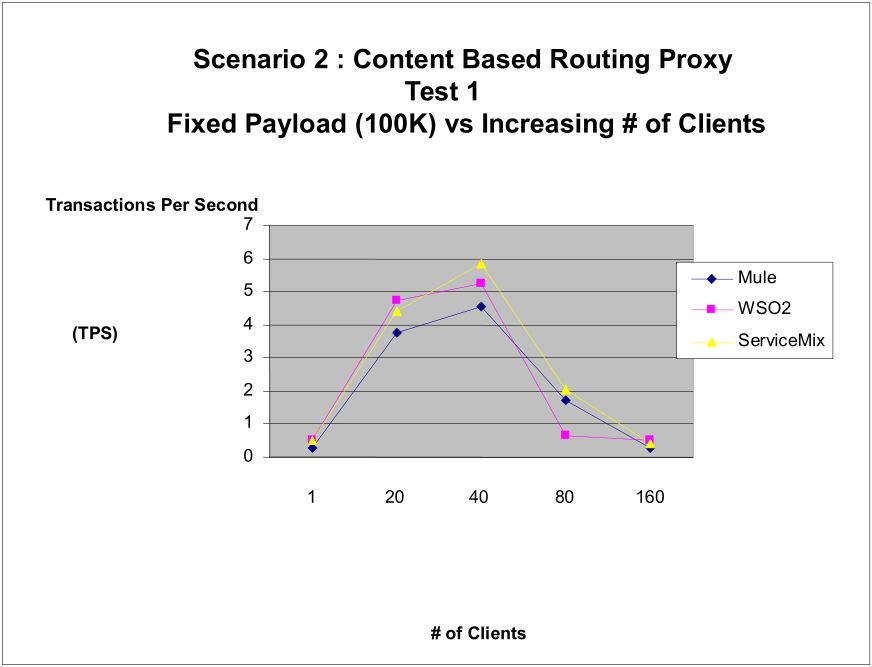
\includegraphics[scale=0.43]{img/Sanjay_cbr_fixed_payload}}
	\label{fig:sanjay_cbr_fixed_payload}
	Using a fixed payload of 100KB and an increasing number of clients the throughput was peaking at 4.5-6 TPS at 40 concurrent clients.

	\caption{Image taken from Sanjay \cite{Sanjay2011} showing their increasing clients content based routing measurements.}
	\centerline{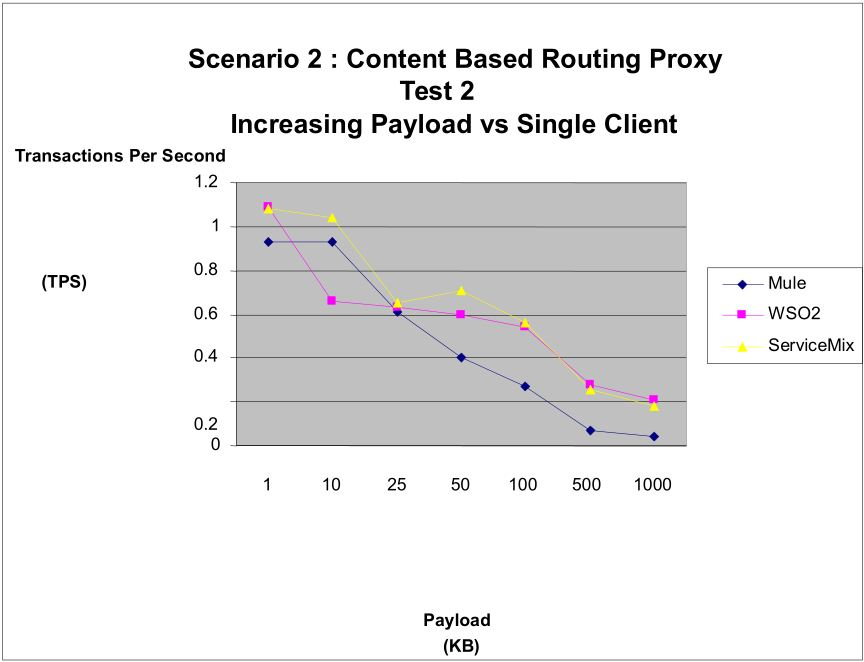
\includegraphics[scale=0.43]{img/Sanjay_cbr_increasing_payload}}
	\label{fig:sanjay_cbr_increasing_payload}
	Single client sending an increasingly larger payload with a TPS between 1.1 and 0.2 which are simply appallingly low numbers.
\end{figure}

When looking at the results from Sanjay \cite{Sanjay2011} in figure \ref{fig:sanjay_cbr_fixed_payload}, \ref{fig:sanjay_cbr_increasing_payload} and the results from WSO2 and Mule \cite{Perera07R3,mulesoft08} in figure \ref{fig:wso2_cbr} and \ref{fig:mule_cbr} one can't help but wonder how Sanjay performed their tests.
Even without the knowledge of the previous tests by WSO2 and Mule their numbers are so low that it seems impossible to consider them as correct yet there is no discussion regarding the validity of the data or their testing procedure. 
It doesn't help that they have not published their hardware setup nor their configuration and ESB source code which means that we cant even begin to hypothezise regarding their data. 


Our results as seen in chapter \ref{test:results} indicate to us that the framework needs more finetuning but that it is a good start for future work. 
The largest contribution done in this thesis is that this could be a starting point for making a testing framework that gives reproducable results and a unified way of testing ESB performance.


%3: future work
One of the more interesting suggestions we would like to make is to include the ESB manufacturers themselves and have them produce the ESB code that is then tested using the framework. 
This would allow a larger number of ESBs to be tested and the code would contain less faults due to the testers inexperience of a particular ESB. 
It would require some secrecy as otherwise the ESB manufacturers could optimize the code in an unnatural manner and that would skew the results.

Recieving optimized code from the manufacturers would also create a baseline that could be used inorder for the tests to be made more advanced and complex.
Increased complexity of the tests could result in more accurate performance tests as the hardware is pushed closer to being maxed out.
Some finetuning of the tools used such as grinder could also be required before the framework should be used on a larger scale.

The configuration files and all source code used in the framework can be found on github at https://github.com/Datanizze/korsdrag-thesis-files